%!TEX root = ../DeGaulle.tex
\section*{Figures}


\begin{figure}[htbp]
 \centering
 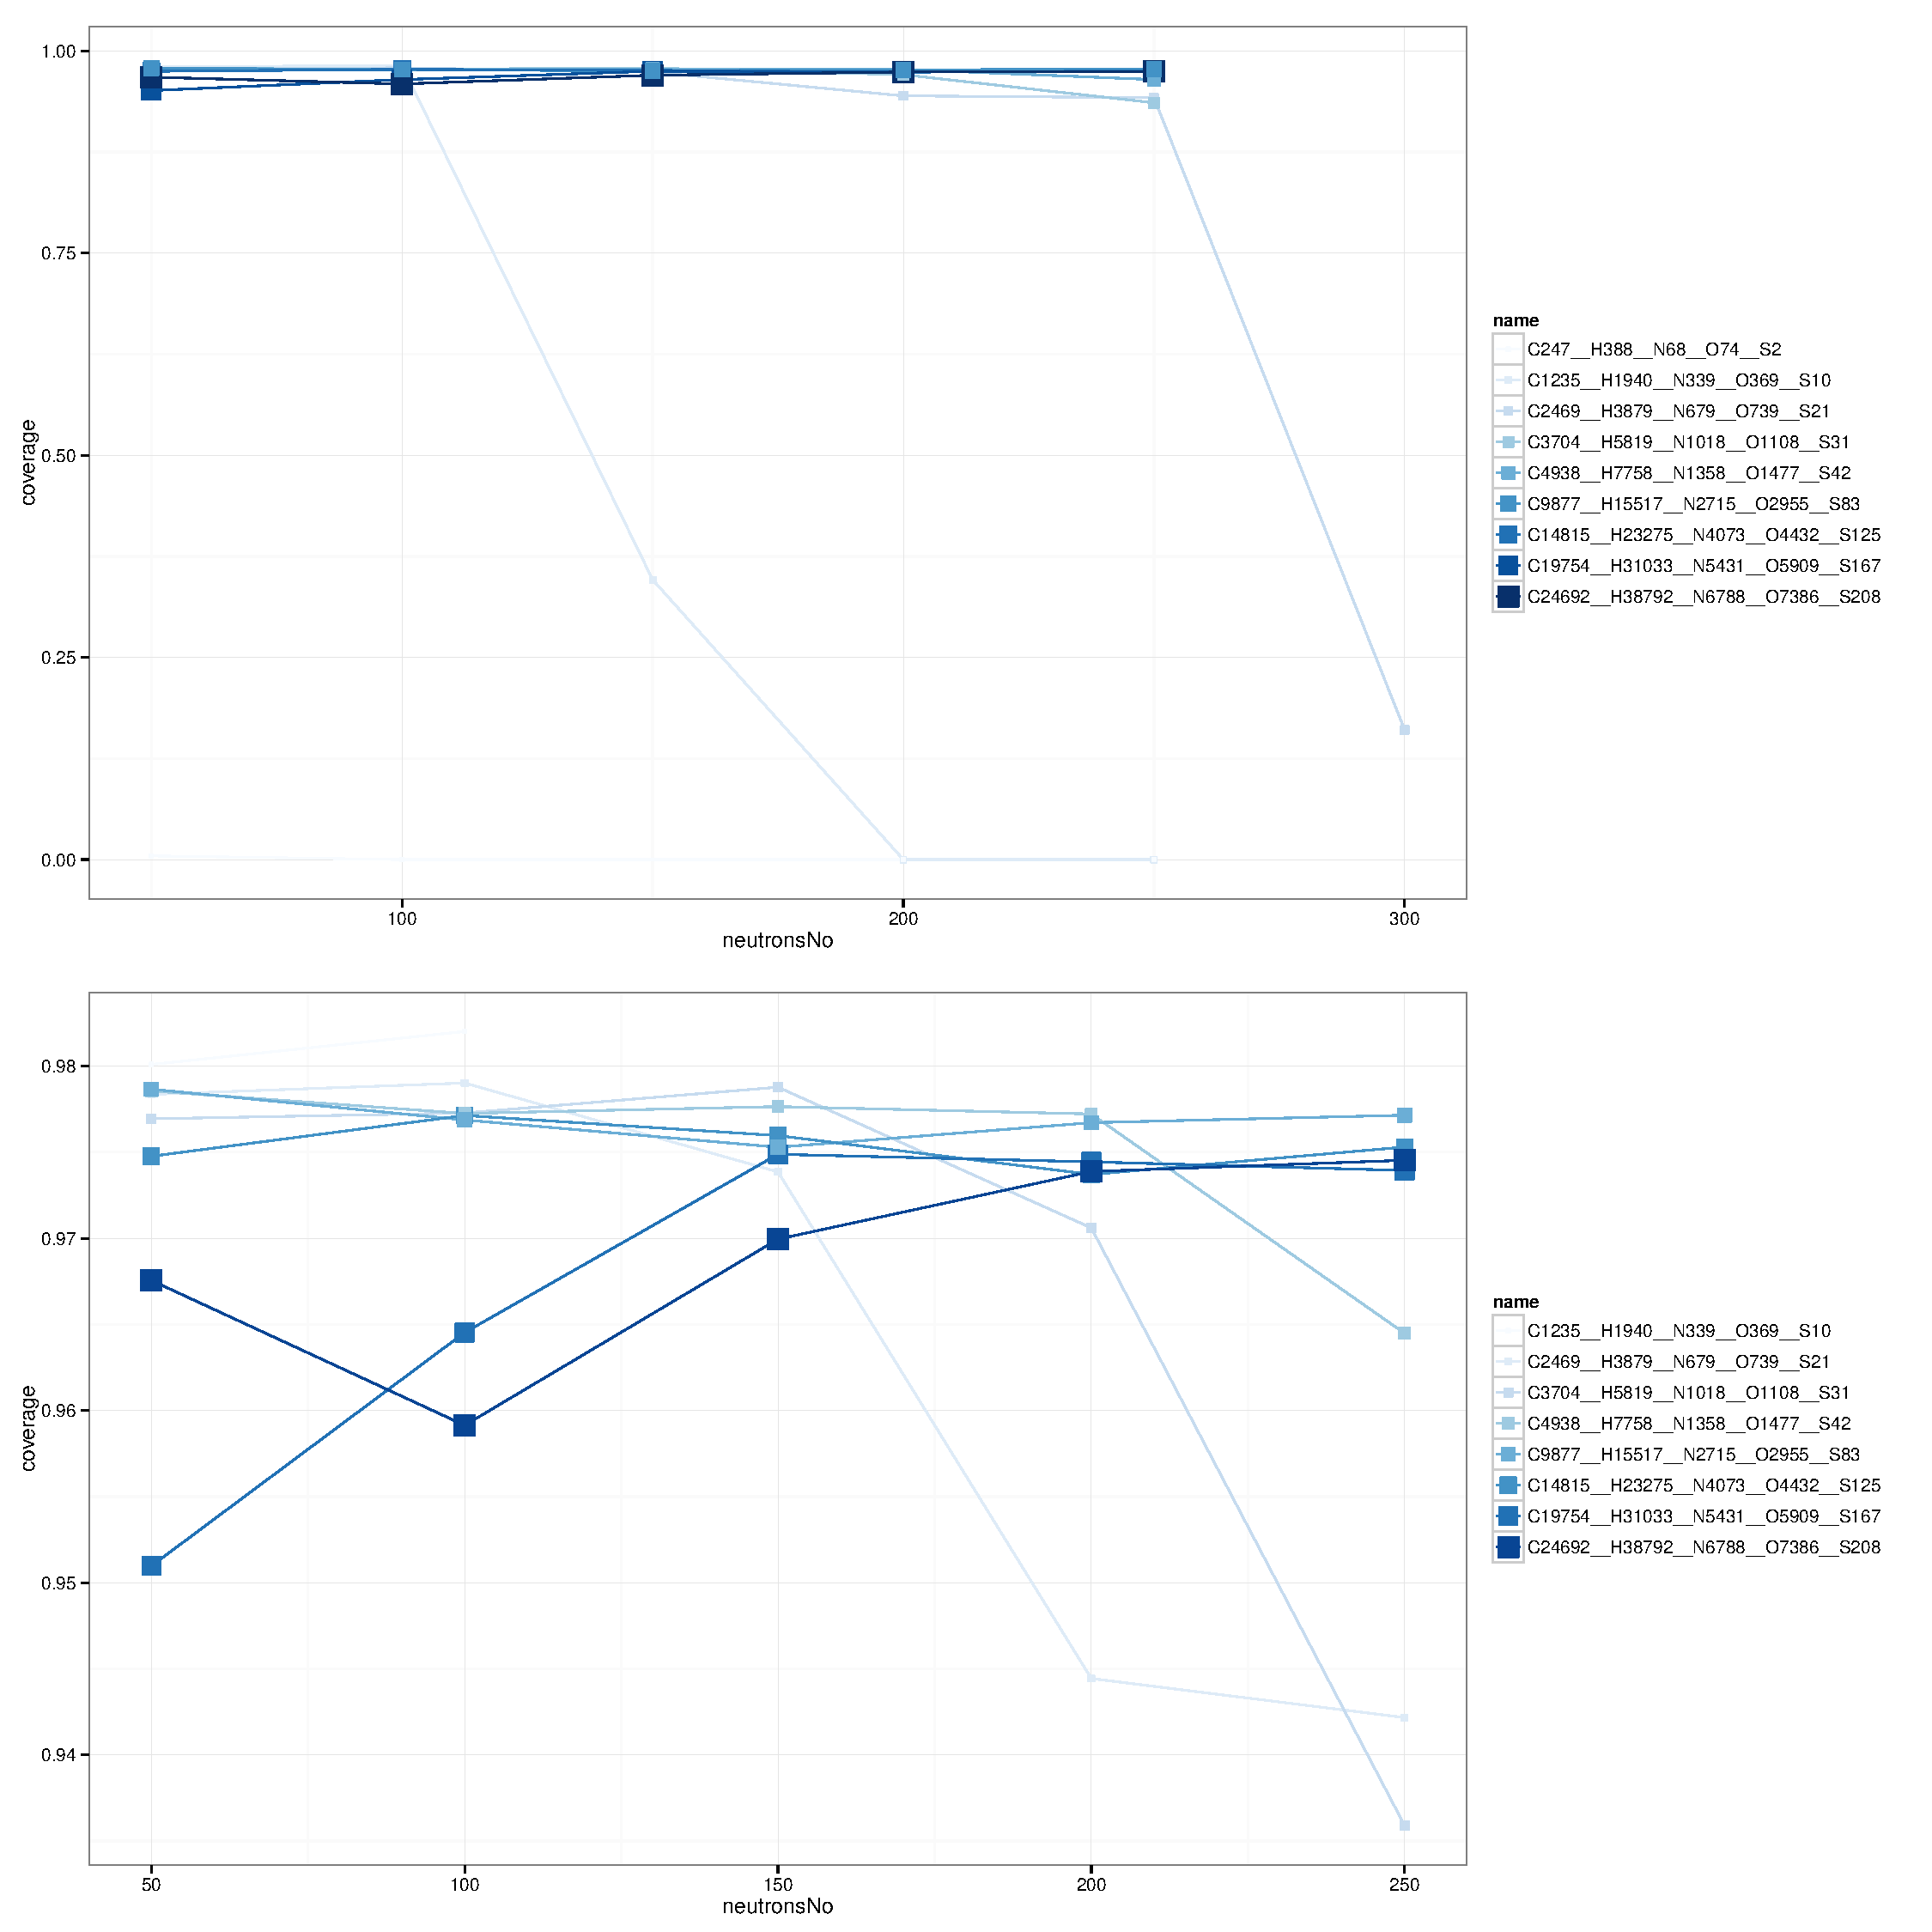
\includegraphics[width=.8\textwidth]{./img/DeFineCoverage}
 \caption{Coverage obtained using {\sc DeFine} algorithm. The image on the bottom zooms into the upper reaches of the top picture. Both show the coverage of distribution original distribution $\MK$ for $K \in \{50, 100, 150, 200, 250, 300 \}$ for several chemical compounds. The bigger the compound (empirical formulas in the legend) the bigger the squares and the more intense the colour. Observe that for lighter compounds the results do not seem promising: we attribute this to the overall quality of conditional distributions $\MK$. Simply, all the multinomial distribution in \eqref{product of multinomials} are unimodal and for larger $K$ the solutions to Diophantine equation \eqref{LFS_K} do not encompass the region next to the mode, where the distribution is centered. For the reasons exposed in \textbf{Conclusions}, it is impractical to look at these distribution in the first place.}
 \label{figure: Coverage}
\end{figure}

